%Use one of the two documentclass lines depending on aspect ratio needed
% for 4x3 aspect ratio slides
%\documentclass{beamer}
%for 16x9 (modern wide screen) aspect ratio slides
\documentclass[aspectratio=169]{beamer}

% Oxford Maths theming
\usetheme{oxfordmaths}

% Set author etc info
\title[Multi-Level Monte Carlo for SPDEs] %short version of title for slide footer
{Multi-Level Monte Carlo Methods for SPDEs} %full title for titlepage
\author{Inti Mantripp}
\institute{Mathematical Institute\\University of Oxford}
\date[6 June 2025]  %short date for slide footer
{MMSC Dissertation Presentations, June 2025} %main date for title page,
                        %can overload it to show say 'Conference X, Date Y'


%% Now for the actual slides %%
\begin{document}

\begin{frame}[plain]
  \titlepage
\end{frame}

\begin{frame}
  \frametitle{Motivating Example: Stochastic Heat Equation}
  \begin{columns}
    \column{0.5\textwidth}
    \textbf{SPDE:} additive noise model
    \[
    \frac{\partial u}{\partial t} = \frac{\partial^2 u}{\partial x^2} + \sigma \xi(x,t)
    \]
    \vspace{1em}
    where:
    \begin{itemize}
      \item \( u(x,t) \) is the solution (random field)
      \item \( \xi(x,t) \) is space-time white noise
      \item \( \sigma \) controls noise amplitude
    \end{itemize}

    \vspace{1em}
    \textbf{Why study this?}
    \begin{itemize}
      \item Arises in physical systems with thermal or environmental randomness
      \item Captures uncertainty and variability in diffusion processes
    \end{itemize}

    \column{0.45\textwidth}
    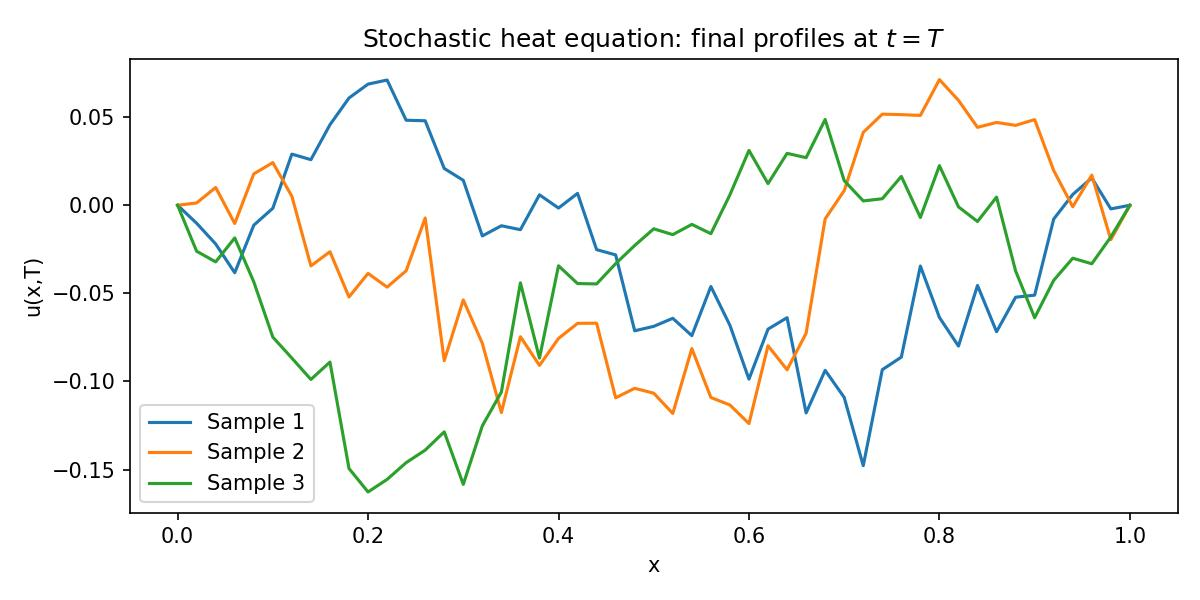
\includegraphics[width=\textwidth]{graphics/stochastic_heat_equation_intro.jpeg}
    \vspace{0.5em}
    \small Illustration: sample profiles of \( u(x,T) \) at final time $T$.
  \end{columns}

  \vspace{1em}
  \textbf{Quantities of interest:}
  \begin{itemize}
    \item Mean field \( \mathbb{E}[u(x,t)] \)
    \item Pointwise variance or confidence intervals
    \item Probability of threshold events, e.g., \( \mathbb{P}(u(x,t) > c) \)
  \end{itemize}

\end{frame}

\begin{frame}
  \frametitle{MLMC Approach to Solving the Stochastic Heat Equation}
  \framesubtitle{From standard Monte Carlo to Multi-Level Monte Carlo}

  \begin{itemize}
    \item To estimate expectations like \( \mathbb{E}[u(x,T)] \) or \( \mathbb{E}\left[\int_0^1 u(x,T)^2 \, dx\right] \), we can use standard Monte Carlo (MC):
    \begin{itemize}
      \item Simulate many independent sample paths of the SPDE
      \item Average the results to estimate expectations
    \end{itemize}

    \pause

    \item \textbf{But}: Monte Carlo convergence is slow — error decreases like \( O(N^{-1/2}) \)

    \pause

    \item \textbf{MLMC (Multi-Level Monte Carlo)} reduces the cost for the same accuracy:
    \begin{itemize}
      \item Simulate cheap, coarse approximations in bulk
      \item Use finer, more expensive simulations sparingly
      \item Combine them to get a more efficient estimator
    \end{itemize}

    \pause

    \item For the stochastic heat equation, this means solving on multiple space-time grids and carefully coupling the noise
  \end{itemize}
\end{frame}

\begin{frame}{Make Titles Informative}
  % - A title should summarize the slide in an understandable fashion
  % for anyone how does not follow everything on the slide itself.
  
\begin{columns}
  \column{0.55\textwidth}
  % Your explanatory bullet points go here

  \column{0.4\textwidth}
  \textbf{Standard Monte Carlo:}
  \[
    \mathbb{E}[P] \approx \frac{1}{N} \sum_{i=1}^N P^{(i)}
  \]
  \[
    \text{Cost: } N \cdot \text{(cost per sample)} \sim \varepsilon^{-2} \cdot \varepsilon^{-2}
  \]
  \[
    = \boxed{O(\varepsilon^{-4})}
  \]

  \vspace{1em}

  \textbf{Multi-Level Monte Carlo:}
  \[
    \mathbb{E}[P_L] = \sum_{\ell=0}^L \mathbb{E}[P_\ell - P_{\ell-1}]
  \]
  \[
    \approx \sum_{\ell=0}^L \frac{1}{N_\ell} \sum_{i=1}^{N_\ell} 
    \big( P_\ell^{(i)} - P_{\ell-1}^{(i)} \big)
  \]
  \[
    \text{Cost: } \boxed{O(\varepsilon^{-2})}
  \]
\end{columns}
\end{frame}


\begin{frame}
  \frametitle{What Are SPDEs? And Why Are They Hard?}

  \begin{itemize}
    \item \textbf{Stochastic partial differential equations (SPDEs)} model the evolution of systems under spatial and temporal uncertainty:
    \[
      \frac{\partial u}{\partial t} = \mathcal{L} u + f(u, x, t) + \text{noise}
    \]
    where the noise may be spatially correlated, time-dependent, or both (e.g. space-time white noise).

    \item \textbf{Analytical difficulties} arise because many SPDEs lack classical solutions:
    \begin{itemize}
      \item Noise is often modelled as a generalised function (e.g. white noise), requiring weak or mild formulations.
      \item Nonlinearities and multiplicative noise may lead to ill-posedness or singular behaviour.
    \end{itemize}

    \item \textbf{Example: The Dean–Kawasaki equation} (a parabolic SPDE modelling stochastic particle densities):
    \[
      \partial_t \rho = \frac{1}{2} \Delta \rho + \nabla \cdot (\rho \nabla V * \rho) + \frac{1}{\sqrt{N}} \nabla \cdot (\sqrt{\rho} \, \xi)
    \]
    \begin{itemize}
      \item Features multiplicative, space-time white noise.
      \item No known strong or mild solution theory; interpreted only via the law of particle systems.
      \item Numerical methods target expected values of functionals rather than trajectories.
    \end{itemize}
  \end{itemize}
\end{frame}

\begin{frame}
  \frametitle{MLMC for SPDEs: Method and Complexity}

  \begin{itemize}
    \item Let \( u \) be the solution to an SPDE and let \( Q(u) \in \mathbb{R} \) be a functional of interest, e.g.
    \[
      Q(u) = \int_D u(x,T)^2 \, dx
    \]

    \item Introduce a sequence of approximations \( Q_\ell := Q(u_\ell) \), where \( u_\ell \) is the numerical solution on grid level \( \ell \), with mesh size \( h_\ell \sim 2^{-\ell} \)

    \item The MLMC estimator:
    \[
      \mathbb{E}[Q_L] = \sum_{\ell = 0}^L \mathbb{E}[Q_\ell - Q_{\ell-1}]
    \quad \text{with } Q_{-1} := 0
    \]
    \[
      \hat{Q}_{\text{MLMC}} := \sum_{\ell=0}^L \frac{1}{N_\ell} \sum_{i=1}^{N_\ell} \left( Q_\ell^{(i)} - Q_{\ell-1}^{(i)} \right)
    \]

    \item Sample costs \( C_\ell \sim h_\ell^{-\gamma} \), variances \( V_\ell := \mathbb{V}[Q_\ell - Q_{\ell-1}] \sim h_\ell^\beta \), and bias \( \sim h_L^\alpha \)

    \item Under conditions \( \beta > \gamma \), the MLMC estimator achieves:
    \[
      \boxed{\text{Total Cost} = O(\varepsilon^{-2}) \quad \text{to achieve RMSE } \leq \varepsilon}
    \]
  \end{itemize}
\end{frame}

\begin{frame}
  \frametitle{MLMC for SPDEs: Method and Variance}

  \begin{itemize}
    \item Let \( u \) solve an SPDE and \( Q(u) \in \mathbb{R} \) be a quantity of interest (e.g., energy functional).
    \item Define approximations \( Q_\ell := Q(u_\ell) \), where \( u_\ell \) is the numerical solution at level \( \ell \).
    \item The MLMC identity:
  \end{itemize}

  \[
    \mathbb{E}[Q_L] = \sum_{\ell=0}^L \mathbb{E}[Q_\ell - Q_{\ell-1}], \quad Q_{-1} := 0
  \]

  \begin{itemize}
    \item Each term is estimated via Monte Carlo:
  \end{itemize}

  \[
    Y_\ell := \frac{1}{N_\ell} \sum_{i=1}^{N_\ell} \left( Q_\ell^{(i)} - Q_{\ell-1}^{(i)} \right)
  \]

  \begin{itemize}
    \item The total MLMC estimator is \( \sum_{\ell=0}^L Y_\ell \), with variance:
  \end{itemize}

  \[
    \mathbb{V}[\hat{Q}_{\text{MLMC}}] = \sum_{\ell=0}^L \frac{V_\ell}{N_\ell}, \quad V_\ell := \mathbb{V}[Q_\ell - Q_{\ell-1}]
  \]

  \begin{itemize}
    \item Optimal sample sizes: \( N_\ell \propto \sqrt{V_\ell / C_\ell} \), where \( C_\ell \sim h_\ell^{-\gamma} \)
    \item Under assumptions:
  \end{itemize}

  \[
    \text{Bias} \sim h_L^\alpha, \quad V_\ell \sim h_\ell^\beta, \quad C_\ell \sim h_\ell^{-\gamma}
  \]

  \begin{itemize}
    \item Then MLMC achieves:
  \end{itemize}

  \[
    \boxed{\text{Cost}_{\text{MLMC}} = O(\varepsilon^{-2}) \quad \text{if } \beta > \gamma}
  \]

\end{frame}


\end{document}
